\chapter{MacroRay Three-Dimensional Ray-tracing Technique}{\label{ch:MacroRay}
  %%% Multi-group Energy quantities %%%
\DeclareDocumentCommand{\gprime}{}{g^{\prime}}
% Cross-sections
\DeclareDocumentCommand{\xs}{ O{t} O{\loc} O{g}}{\ensuremath{\CrossSection_{#1}^{#3}(#2)}}
\DeclareDocumentCommand{\xst}{ O{\loc} O{g} }{\xs[t][#1][#2]}
\DeclareDocumentCommand{\xsa}{ O{\loc} O{g} }{\xs[a][#1][#2]}
\DeclareDocumentCommand{\xsf}{ O{\loc} O{\gprime} }{\xs[f][#1][#2]}
\DeclareDocumentCommand{\xss}{ o O{\loc} O{\dirprime\vdot\dir} O{\gprime \to g} }{
    \IfNoValueOrEmptyTF{#1}
    {\xs[s][#2,#3][#4]}
    {\xs[s,#1][#2][#4]}
}
\DeclareDocumentCommand{\spect}{ O{\loc} O{g} }{\ensuremath{\Spectrum^{#2}(#1)}}
\DeclareDocumentCommand{\nufis}{ O{\loc} O{\gprime} }{ \ensuremath{\nu\xsf[#1][#2]}}
\DeclareDocumentCommand{\D}{ O{\loc} O{g} }{\ensuremath{D^{#2}(#1)}}

% Flux
\DeclareDocumentCommand{\aflux}{ O{\loc} O{\dir} O{g} }{\ensuremath{\AngularFlux^{#3}(#1,#2)}}
\DeclareDocumentCommand{\sflux}{ O{\loc} O{\gprime} }{\ensuremath{\ScalarFlux^{#2}(#1)}}
\DeclareDocumentCommand{\current}{ O{\loc} O{g} }{\ensuremath{\Current^{#2}(#1)}}
\DeclareDocumentCommand{\fluxmoma}{ O{\ell} O{n} O{\loc} O{g} }{\ensuremath{\ScalarFlux^{#2,#4}_{#1}(#3)}}

% Source
\DeclareDocumentCommand{\source}{ O{\loc} O{\dir} O{g} }{\ensuremath{q^{#3}(#1,#2)}}
\DeclareDocumentCommand{\sourcemoma}{ O{\ell} O{n} O{\loc} O{g} }{\ensuremath{q^{#2,#4}_{#1}(#3)}}

  %%% Discrete Ordinates Quantities %%%
\DeclareDocumentCommand{\mprime}{}{m^{\prime}}
\DeclareDocumentCommand{\dirm}{ O{m} }{\dir_{#1}}
\DeclareDocumentCommand{\wt}{ O{m} }{\Weight_{#1}}

% Quadrature set
\DeclareDocumentCommand{\angquad}{ O{N} }{ \mathcal{M}_{#1} }

% Cross-Sections
\DeclareDocumentCommand{\xss}{ o O{\loc} O{ m^{\prime}\!\to m} O{\gprime\!\to g} }{
    \IfNoValueOrEmptyTF{#1}
    {\xs[s,#3][#2][#4]}
    {\xs[s,#1][#2][#4]}
}

% Flux
\DeclareDocumentCommand{\aflux}{ O{\loc} O{m} O{g}}{\ensuremath{\AngularFlux^{#3}_{#2}\!\left(#1\right)}}

% Source
\DeclareDocumentCommand{\source}{ O{\loc} O{m} O{g} }{\ensuremath{q^{#3}_{#2}\!\left(#1\right)}}

  %%% MOC quantities %%%
% Geometric
\DeclareDocumentCommand{\Length}{}{s}
\DeclareDocumentCommand{\NormalizedLength}{}{t}
\DeclareDocumentCommand{\len}{ O{} }{\Length_{#1}}
\DeclareDocumentCommand{\segl}{ O{mki} }{\Length_{#1}}
\DeclareDocumentCommand{\nlen}{ O{m} }{\NormalizedLength_{#1}}
\DeclareDocumentCommand{\nsegl}{ O{mki} }{\NormalizedLength_{#1}}

\DeclareDocumentCommand{\centroid}{ O{\loc} O{i} }{#1_{#2}^{\text{c}}}
\DeclareDocumentCommand{\locIn}{ O{\loc} O{mki} }{{#1}_{#2}^{\text{in}}}
\DeclareDocumentCommand{\locOut}{ O{\loc} O{mki} }{{#1}_{#2}^{\text{out}}}
\DeclareDocumentCommand{\locCent}{ O{\loc} O{mki} }{{#1}_{#2}^{\text{c}}}
\DeclareDocumentCommand{\M}{ o O{i}}{%
    \IfNoValueOrEmptyTF{#1}
        {\vec{M}_{#2}}
        {M_{#2,#1}}
}
\DeclareDocumentCommand{\C}{o O{i} O{g}}{%
    \IfNoValueOrEmptyTF{#1}
        {\vec{C}_{#2}^{#3}}
        {C_{#2,#1}^{#3}}
}


% Integration
\DeclareAutoPairedDelimiter{\MOCTrackIntegral}{\langle}{\rangle_{mki}}
\DeclareAutoPairedDelimiter{\MOCSingleAngleIntegral}{\langle}{\rangle_{mi}}
\DeclareAutoPairedDelimiter{\MOCIntegral}{\langle}{\rangle_{i}}

% Cross-sections
\DeclareDocumentCommand{\xs}{ O{t} O{i} O{g}}{\ensuremath{\CrossSection_{#1,#2}^{#3}}}
\DeclareDocumentCommand{\xst}{ O{i} O{g} }{\xs[t][#1][#2]}
\DeclareDocumentCommand{\xsa}{ O{i} O{g} }{\xs[a][#1][#2]}
\DeclareDocumentCommand{\xsf}{ O{i} O{\gprime} }{\xs[f][#1][#2]}
\DeclareDocumentCommand{\xss}{ o O{i} O{m'\to m} O{\gprime \to g} }{
    \IfNoValueOrEmptyTF{#1}
    {\xs[s][#2,#3][#4]}
    {\xs[s,#1][#2][#4]}
}

\DeclareDocumentCommand{\spect}{ O{i} O{g} }{\ensuremath{\Spectrum^{#2}_{#1}}}
\DeclareDocumentCommand{\nufis}{ O{i} O{\gprime} }{ \ensuremath{\nu\xsf[#1][#2]}}
\DeclareDocumentCommand{\D}{ O{i} O{g} }{\ensuremath{D^{#2}_{#1}}}
\DeclareDocumentCommand{\opt}{ O{m} O{g} }{\OpticalThickness_{#1}^{#2}}
\DeclareDocumentCommand{\segopt}{ O{mki} O{g} }{\opt[#1][#2]}

% MOC Parameters
\DeclareDocumentCommand{\tA}{ O{a} }{\ensuremath{\delta\!A_{#1}}}
\DeclareDocumentCommand{\Weight}{}{w}
\DeclareDocumentCommand{\wt}{ O{m} }{\Weight_{#1}}
\DeclareDocumentCommand{\wtbar}{ O{m} }{\overline{\Weight}_{#1}}
\DeclareDocumentCommand{\renorm}{ O{i} }{\ensuremath{\xi_{#1}}}

% Flux
\DeclareDocumentCommand{\aflux}{ O{mki} O{g} O{\len} }{
    \IfNoValueOrEmptyTF{#3}
    {\AngularFlux^{#2}_{#1}}
    {\ensuremath{\AngularFlux^{#2}_{#1}\!\left(#3\right)}}
}
\DeclareDocumentCommand{\afluxin}{ O{mki} O{g} }{\AngularFlux^{#2,\text{in}}_{#1}}
\DeclareDocumentCommand{\afluxout}{ O{mki} O{g} }{\AngularFlux^{#2,\text{out}}_{#1}}
\DeclareDocumentCommand{\sflux}{ O{g} O{i} }{\ScalarFlux_{#2}^{#1}}
\DeclareDocumentCommand{\current}{ O{i} O{g} }{\Current^{#2}_{#1}}
\DeclareDocumentCommand{\tfluxF}{ O{mki} O{g} }{ \overline{\AngularFlux}_{#1}^{#2} }          % Average flux-moment along track
\DeclareDocumentCommand{\tfluxL}{ O{mki} O{g} }{  \widehat{\AngularFlux}_{#1}^{#2} }          % Linear flux-moment along track
\DeclareDocumentCommand{\dflux}{ O{mki} O{g} }{ \Delta\AngularFlux_{#1}^{#2} }                % Difference of angular flux along track
\DeclareDocumentCommand{\sfluxF}{ O{i} O{g} }{ \overline{\ScalarFlux}_{#1}^{#2} }             % Average scalar flux
% \DeclareDocumentCommand{\sfluxL}{ o O{i} O{g} }{ % Linear expansion coeff (Scalar Flux)
%     \IfNoValueOrEmptyTF{#1}
%         {\lvec{\widehat{\ScalarFlux}}_{#2}^{#3}}
%         {\widehat{\ScalarFlux}_{#2,#1}^{#3}}
% }
\DeclareDocumentCommand{\sfluxL}{ O{i} O{g} o }{ % Linear expansion coeff (Scalar Flux)
    \IfNoValueOrEmptyTF{#3}
        {\lvec{\widehat{\ScalarFlux}}_{#1}^{#2}}
        {\widehat{\ScalarFlux}_{#1,#3}^{#2}}
}
% \DeclareDocumentCommand{\sfluxL}{ m O{i} O{g} }{\widehat{\ScalarFlux}_{#2,#1}^{#3} }          % Linear expansion coeff (Scalar flux)
\DeclareDocumentCommand{\afluxmom}{ O{\ell} O{n} O{i} O{\gprime} }{\FluxMoment_{#3,#1}^{#4,#2}}

% Source
\DeclareDocumentCommand{\source}{ O{mki} O{g} O{\len} }{\ensuremath{q^{#2}_{#1}\!\left(#3\right)}}
\DeclareDocumentCommand{\tsrcF}{ O{mki} O{g} }{ \overline{q}_{#1}^{#2} }          % Average source along track
\DeclareDocumentCommand{\tsrcL}{ O{mi} O{g} }{ \widehat{q}_{#1}^{#2} }          % Linear source along track
\DeclareDocumentCommand{\src}{ O{i} O{g} }{ \Source_{#1}^{#2}}                          % Generic source
\DeclareDocumentCommand{\srcF}{ O{i} O{g} }{ q_{#1}^{#2} }             % Average source
\DeclareDocumentCommand{\srcL}{ o O{i} O{g} }{ % Linear expansion coeff (Source)
    \IfNoValueOrEmptyTF{#1}
        {\lvec{\widehat{q}}_{#2}^{#3}}
        {\widehat{q}_{#2,#1}^{#3}}
}

% Linear source operators / functions
\DeclareDocumentCommand{\FluxToSource}{ O{g} }{\mathcal{S}^{#1}}
  \def\figpath{chapters/MacroRay/figures/}
  \graphicspath{ {\figpath} }

  The primary motivation of the three-dimensional macroray ray-tracing technique is to reduce the number of tracks generated for 3-D \ac{MOC} applications.
  The number of track-segments is very strongly correlated with the run-time of a \ac{MOC} calculation \footnote{if the \ac{MOC} calculation performs an entirely separate calculation (i.e does not use the chord-classification method) for each track-segment, this is expected to be directly proportional (ignoring overhead)}.
  The 2-D macroband ray-tracing method had been shown to allow for coarser ray-spacing compared to traditional methods, but it has never been extended for use in 3-D \ac{MOC} calculations.
  This work seeks to fill that gap, and perform an investigation into the extension from 2-D to 3-D macroband-like ray-tracing.
  The ray-tracing technique is referred to as the \emph{macroray}, because the 3-D ``macro''paths are no longer bands, but instead parallel-pipes.

  This work implemented a 3-D ray-tracing and transport solver library in MPACT based on the macroray method.
  The initial step in this implementation was to implement a 2-D version \footnote{which does not currently support \ac{CMFD} acceleration}.
  This also serves to confirm the results of previous studies on 2-D macroband \cite{Yamamoto2005,Fevotte2007}.

  \section{MacroRay Technique}{\label{sec:MR:MacroRay Technique}
    The macroray ray-tracing technique is a 3-D extension of the macroband method; in order to describe this new ray-tracing technique it is first necessary to describe the macroband method.
    \Cref{ssec:RT:Macroband} gave a brief summary of the history of macroband, as well as some benefits of the method.
    This section will describes the macroband method in more detail, and shows how the method is extended to 3-D.

    \subsection{Macroband Technique}{\label{ssec:MR:Macroband Technique}
      The macroband was first used in the \acf{CP} code HELIOS, and was considered to be essential for the stability of the method \cite{Villarino1992}.
      Unlike the traditional uniform/equidistant ray-tracing methods, the macroband method guarantees that each ray within a macroband will pass through the same regions in the same sequence, and not have any regions within its bounds that are not crossed by the rays.
      This means that the placement of rays, and their widths, are determined by the internal geometry of the pin or subdomain that is being traced.
      Each ray within a macroband passes through the same regions albeit with different lengths; if the incident flux for the macroband is smooth, this means that the track-segment average flux will also be smooth.
      This allows for the use of more advanced transverse integration, such as Gauss-Legendre quadrature integration \cite{Yamamoto2005}.
      A similar method was also developed by \citet{Fevotte2007} where coarse equidistant ray calculations were performed by using a macroband approach within the ray's transverse area (with a single ray per band).

      The macroband method ray-tracing is described in \cref{alg:Macroband:Ray-tracing}.
      A downside of this method is that each ray has a unique width that requires additional storage.
      However, all rays within a macroband pass through the same segments, so the region index for each segment only needs to be stored once, reducing memory by a larger amount.
      The process is shown visually in \cref{fig:MR:Macroband Process}.

      \begin{algorithm}[ht]
        \centering
        \caption{Macroband ray-tracing procedure for a pin-cell.\label{alg:Macroband:Ray-tracing}}
        \begin{algorithmic}[1]
          \State{Begin with a pin-cell geometry/mesh, and a direction of flight $\dirm$.}
          \State{Create a list of points, $P$, containing:
            \begin{enumerate}
              \item{corners,}
              \item{mesh intersections,}
              \item{and tangent points.}
            \end{enumerate}
          }
          \State{Sort the points by signed distance in the normal direction, $\widehat{n}_m$, from center of pin}
          \State{The macrobands are bounded in the transverse direction by these distances}
          \ForAll{Macrobands}
            \State{Determine quadrature points and widths in transverse direction}
            \State{Place rays at these points with these widths}
            \State{Trace each ray}
          \EndFor
        \end{algorithmic}
      \end{algorithm}

      \begin{figure}[ht]
        \centering
        \begin{subfigure}[t]{0.33\linewidth}
          \centering
          \def\svgwidth{0.95\linewidth}
          \input{\figpath/Macroband/MacroBandProcess1.pdf_tex}
          \caption{Determine intersection and tangent points}
        \end{subfigure}%
        \hfill
        \begin{subfigure}[t]{0.33\linewidth}
          \centering
          \def\svgwidth{0.95\linewidth}
          \input{\figpath/Macroband/MacroBandProcess2.pdf_tex}
          \caption{Determine macroband boundaries (through identified points)}
        \end{subfigure}%
        \hfill
        \begin{subfigure}[t]{0.33\linewidth}
          \centering
          \def\svgwidth{0.95\linewidth}
          \input{\figpath/Macroband/MacroBandProcess3.pdf_tex}
          \caption{Perform ray-tracing within macroband boundaries}
        \end{subfigure}
        \caption{Ray-tracing process for macroband.}
        \label{fig:MR:Macroband Process}
      \end{figure}

      As it is difficult to visualize 3-D ray-tracing data in a 2-D textual media, a quarter \ac{IFBA} fuel pin will be used as an example to demonstrate the differences between ray-tracing methods.
      \Cref{figs:MR:Macroband-Single-Visualization,figs:MR:Macroband-All-Visualization} compare the traditional \ac{MRT} ray-tracing technique with the macroband method with Gauss-Legendre spacing.
      The rays for a single direction make it clear that the \ac{MRT} in no way accounts for the internal geometry.
      In the macroband method, there are clearly regions that have more rays passing through them; in this case, it is the boron layer coating the fuel.
      When all directions are visualized, again the \ac{MRT} would use this same pattern of rays whether this was an \ac{IFBA} rod, or a rectangular reflector (of the same size).
      In the macroband methods, some of the geometry becomes very apparent, the outline of the pin can clearly be seen due to the methods forcing rays through the thin coating.

      \begin{figure}[htbp]
        \centering
        \begin{subfigure}[t]{0.33\textwidth}
          \centering
          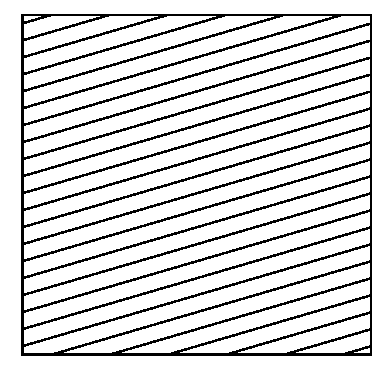
\includegraphics[width=0.9\textwidth]{\figpath/Macroband/MRT-single}
          \caption{MRT}
        \end{subfigure}%
        ~
        \begin{subfigure}[t]{0.33\textwidth}
          \centering
          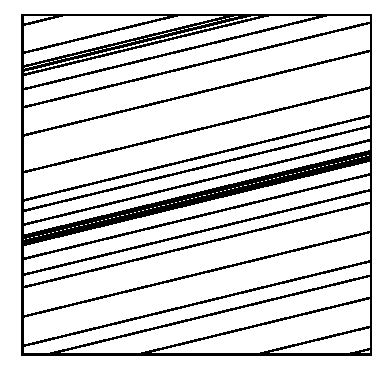
\includegraphics[width=0.9\textwidth]{\figpath/Macroband/MBGL-single}
          \caption{Macroband (Gauss-Legendre)}
        \end{subfigure}
        \caption{2-D single angle ray-tracing comparison for quarter IFBA pin. \label{figs:MR:Macroband-Single-Visualization}}
      \end{figure}

      \begin{figure}[htbp]
        \centering
        \begin{subfigure}[t]{0.49\textwidth}
          \centering
          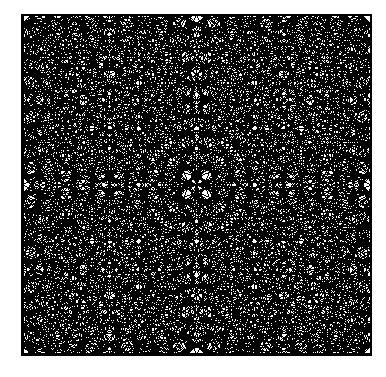
\includegraphics[width=0.95\textwidth]{\figpath/Macroband/MRT-all}
          \caption{MRT}
        \end{subfigure}%
        ~
        \begin{subfigure}[t]{0.49\textwidth}
          \centering
          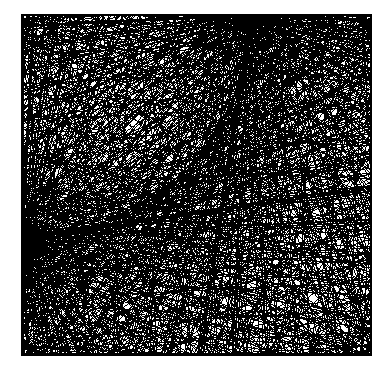
\includegraphics[width=0.95\textwidth]{\figpath/Macroband/MBGL-all}
          \caption{Macroband (Gauss-Legendre)}
        \end{subfigure}
        \begin{subfigure}[t]{0.49\textwidth}
          \centering
          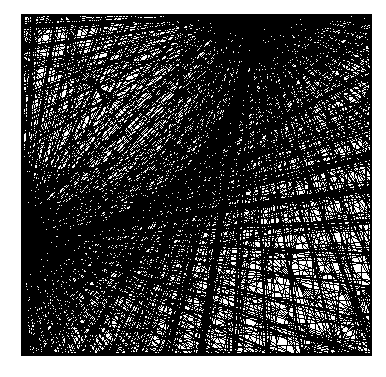
\includegraphics[width=0.95\textwidth]{\figpath/Macroband/MBGL-fixed-all}
          \caption{Macroband-fixed (Gauss-Legendre)}
        \end{subfigure}
        \caption{2-D ray-tracing comparison for quarter IFBA pin. \label{figs:MR:Macroband-All-Visualization}}
      \end{figure}
    }
    There have been different approaches to 3-D ray-tracing for \ac{MOC}; the most common approach is to first generate 2-D tracking data, forming characteristic planes.
    Then 2-D tracking data is generated for each of the characteristic planes.
    This process was described in detail in \cref{ssec:RT:Three-Dimensional Ray-Tracing Techniques}, and will be referred to as the 2D/2D ray-tracing approach.
    This was the approach taken for this thesis work, but other approaches may have significant advantages; these will be discussed in \cref{ssec:MR:Interface Angular Flux Approximation}.

    Although previous works have investigated the 2-D macroband ray-tracing method \cite{Yamamoto2005,Fevotte2007,Yamamoto2008}, there have not been any studies in the extension of macroband to 3-D \ac{MOC} calculations.
    Here, the macroray ray-tracing technique uses the macroband method for both the 2-D radial track generation, and 2-D track generation within each characteristic plane.
    The setup procedure of the macrorays guarantee that their rays pass through the same regions, just as the macroband's did.
    However, it is no longer guaranteed that any region contained within the volume of a macroray will be traversed by the ray.
    This leads to some issues that are discussed in \cref{ssec:MR:Interface Angular Flux Approximation}.

    Similarly to the macroband method, the macroray method is fundamentally incompatible with the \acf{DNPL} ray-tracing technique \cite{Saji2000}.
    The \acf{MRMB} technique \cite{Yamamoto2005} can be used to store tracking data for unique geometric subsystems (typically a pin cell), greatly reducing memory usage.
    Although tracking data can be generated for unique geometry subsystems (\ac{MRMB} \cite{Yamamoto2005}), some approximation of the angular flux is necessary on interfaces.
    Generally, the macroray and macroband methods, which provide more accurate integration, exchange regional numerical dispersion for interface numerical dispersion \cite{Sanchez2012}.
    It is the point of view of the author that this is generally a favorable trade-off, as the engineering quantities of interest are primarily determined through regional integration.

    \subsection{Chord-Classification}{\label{ssec:MR:Chord-Classification}
      The chord-classification ray-tracing method \cite{Sciannandrone2016} was described in detail in \cref{sssec:RT:Chord-Classification}.
      One of the key criticisms of this method, by \citet{Gunow2018}, was that full 3-D tracking data needed to be generated prior to the classification of rays.
      However, with the addition of the macroray ray-tracing method, classification can be done automatically.

      During the axial ray-tracing along a characteristic plane, the computational mesh is used to determine the axial macrobands.
      Each ray within the macroray is guaranteed to pass through the same regions and surfaces; this means that each ray within an axial macroband is guaranteed to be of the same chord classification.
      This is demonstrated visually in \cref{fig:RT:Chord-Classification Macroray}.
      The chord-classification drastically cuts down on the amount of memory used to store 3-D tracking data, and also may reduce the amount of computational work.
      The work is reduced because the exponential functions (see \cref{sec:LSMOC:Exponential Tabulation}) are determined by the material and segment length.
      For vertical-to-vertical or horizontal-to-horizontal macroray segments, the segment lengths of all rays are the same, thus only a single exponential calculation is necessary.

      The chord-classification approach was taken in this work, rather than on-the-fly ray-tracing \cite{Gunow2018}.
      This was done due to the ease of implementation (since the classification is automatic), and because of the criticisms of on-the-fly ray-tracing described in \cref{ssec:RT:On-the-Fly Ray-Tracing}.

      \begin{figure}[h]
        \centering
        \def\svgwidth{0.45\linewidth}
        \input{\figpath/ChordClassificationMacroBand.pdf_tex}
        \caption{3-D example of chord-classification with Macroray ray-tracing. Colored (red and blue) characteristic tracks represent groups of ``V-chords'', rays between two vertical surfaces.}
        \label{fig:RT:Chord-Classification Macroray}
      \end{figure}
    }

    \subsection{Interface Angular Flux Approximation}{\label{ssec:MR:Interface Angular Flux Approximation}
      In \cref{sssec:RT:Interface Flux Approximations} different approaches to approximating the angular flux on the boundaries were outlined for a 2-D macroband-based \ac{MOC} calculation.
      A ``fraction contribution'' sub-boundary averaging technique was described and chosen as the approach for this work.
      In this approach, each surface of the subsystems (pin cells) is divided into sub-boundaries based on the direction of flight.
      Each ray's width is considered, and partial intersections with each surface are computed and used to determine the ray's fractional contribution to each sub-boundary.
      In the reverse direction (going from sub-boundary to ray), each sub-boundaries fractional contribution to each ray is determined.
      It was shown that this method conserved the total area-integrated angular flux on each surface.

      However, in 3-D this approach becomes considerably more complicated, due to the nature of 3-D geometries and the 2D/2D ray-tracing approach.
      An issue arises from the fact that each ray, as viewed in the direction of flight, is rectangular.
      Each ray is rectangular because in the radial ray-tracing step, the ray is considered within the bounds of the width in the radially transverse direction, and in the axial ray-tracing on the characteristic plane the ray is again constrained in a height in the axially transverse direction.
      The rectangular ray projection is demonstrated for a single ray in \cref{figs:MR:MacroRayProjections}.

      For 3-D extruded cartesian pin cells, it is impossible (in arbitrary directions) to ``span''\footnote{in this context, ``span'' will be used to describe the idea that each ray's entire area projects onto some surface, and the entire surface is filled with ray projections.} the surfaces of our system.
      Because each ray is rectangular, parts of the pin cell's surfaces will not be ``hit'' by the projection of any ray, and parts of some rays will live entirely outside the problem domain.
      This issue is visualized in \cref{fig:MR:MacroRayProjectionProblem}; it should also be noted that the area outside the domain, and the surface area without any covering rays are not equal in area unless the ray is in the center of the radial width.

      \begin{figure}[htbp]
          \centering
          \begin{subfigure}[t]{0.45\textwidth}
              \centering
              \def\svgwidth{0.70\linewidth}
              \input{\figpath/MacroRayProjections.pdf_tex}
              \caption{2-D ray viewed from above\label{fig:MR:MacroRayProjections}}
          \end{subfigure}%
          \begin{subfigure}[t]{0.45\textwidth}
              \centering
              \def\svgwidth{0.70\linewidth}
              \input{\figpath/MacroRayProjectionsDOF.pdf_tex}
              \caption{3-D ray viewed in direction of flight\label{fig:MR:MacroRayProjectionsDOF}}
          \end{subfigure}
          \caption{Example of the projected rectangular area formed in the 2D/2D ray-tracing approach.}
          \label{figs:MR:MacroRayProjections}
      \end{figure}

      \begin{figure}[htbp]
        \centering
        \def\svgwidth{0.25\linewidth}
        \input{\figpath/MacroRayProjectionsDOFProblem.pdf_tex}
        \caption{
            An example of a ray that causes issues with the fractional contribution interface flux approximation when using 2D/2D ray-tracing.
            The highlighted red area is the area of the ray outside the domain (that projects to no surface), and the blue highlighted area is an area on the surface that will not be hit by any ray.}
        \label{fig:MR:MacroRayProjectionProblem}
      \end{figure}

      The rays not ``spanning'' our system causes issues with the conservation of surface flux and leakages as described in \cref{sssec:RT:Interface Flux Approximations}.
      Previously, the average angular flux in a sub-boundary was determined by
      \begin{equation}\label{eq:MR:Old SubBoundary Flux}
        \psi_s^i = \suml[j] \frac{A(S_i\cap R_j)}{A(S_i)}\psi_r^j.
      \end{equation}
      It was shown that by summing over all sub-boundaries, the leakage through the surface was conserved.
      However, because the rays are no longer guaranteed to span the system's surfaces, the summation of intersected ray areas is no longer equal to the sub-boundary areas:
      \begin{equation}\label{eq:MR:Area Imbalance}
        \suml[j] A(S_i\cap R_j) \leq A(S_i).
      \end{equation}
      Generally, these areas are very close, and in the limit of infinite rays they are equivalent; but, the motivation of this work has been to reduce the number of rays, so this issue needs to be addressed.
      \Cref{sssec:MR:MacroRay Area Correction} describes how this issue was addressed in this work, and \cref{sssec:MR:Alternative Approaches} describes possible alternative approaches.

      \subsubsection{MacroRay Area Correction}{\label{sssec:MR:MacroRay Area Correction}
        Two ideas were investigated in order to address the issue of the rays not spanning the surface areas.
        Here, it should be emphasized that the first approach is \emph{incorrect}.
        It is described in this section because it seems like a reasonable choice for this correction; in fact, it was not realized for some time in this work that the first approach was incorrect.

        The sub-boundary averaging method of this work has been referred to as a ``fractional contribution'' approach.
        This comes from \cref{eq:MR:Old SubBoundary Flux} where $A(S_i \cap R_j) / A(S_i)$ is the fractional contribution of flux from ray $j$ into sub-boundary $i$.
        In 2-D, these fractions will sum to one, because our rays span the surfaces of our system:
        \begin{equation}\label{eq:MR:2-D Fractional Unity}
          \suml[j] \frac{A(S_i \cap R_j)}{A(S_i)} = 1.
        \end{equation}

        The first approach taken attempted to preserve this property of fractional contributions summing to unity.
        This is done by ignoring ray areas outside the domain and surface areas that are not covered by ray projections; the sub-boundary and ray fluxes are determined by
        \begin{subequations}\label[subeqs]{eqs:MR:Flux A1}
          \begin{equation}\label{eq:MR:SubBoundary Flux A1}
            \psi_s^i = \suml[j] \frac{A(S_i \cap R_j)}{\suml[k] A(S_i \cap R_k)}\psi_r^j = \suml[j] \frac{A(S_i \cap R_j)}{A_p(S_i)}\psi_r^j,
          \end{equation}
          \begin{equation}\label{eq:MR:Ray Flux A1}
            \psi_r^j = \suml[i] \frac{A(S_i \cap R_j)}{\suml[k] A(S_k \cap R_j)}\psi_s^i = \suml[i] \frac{A(S_i \cap R_j)}{A_p(R_j)}\psi_s^i,
          \end{equation}
        \end{subequations}
        respectively.
        For convenience, let us define the ``total projected area'' as the sum of intersections for that object, for example the total projected area of a ray would be defined by
        \begin{equation}\label{eq:MR:Projected Area Ray}
          A_p(R_j) \defined \suml[i] A(S_i \cap R_j),
        \end{equation}
        and similarly for $A_p(S_i)$.
        Through these definitions the new fractional contributions sum to unity:
        \begin{subequations}\label[subeqs]{eqs:MR:Fractions A1}
          \begin{equation}\label{eq:MR:SubBoundary Fractions A1}
            \suml[j] \frac{A(S_i \cap R_j)}{A_p(S_i)} = 1,
          \end{equation}
          and
          \begin{equation}\label{eq:MR:Ray Fractions A1}
            \suml[i] \frac{A(S_i \cap R_j)}{A_p(R_j)} = 1.
          \end{equation}
        \end{subequations}

        While this may seem reasonable \footnote{at least at first to the author}, this is not actually the property we need to preserve for compatibility with \ac{CMFD} acceleration.
        The leakage needs to be preserved, but in this first approach this is not the case.
        \begin{subequations}\label[subeqs]{eqs:MR:Flux Conservation A1}
          \begin{equation}\label{eq:MR:SubBoundary Flux Conservation A1}
            L^s = \dir\vdot\vec{\hat{n}}\suml[i] A(S_i) \psi_s^i
                     = \dir\vdot\vec{\hat{n}} \suml[i] A(S_i) \suml[j] \frac{A(S_i \cap R_j)}{A_p(S_i)}\psi_r^j
                     \neq \psi_t^r,
          \end{equation}
          \begin{equation}\label{eq:MR:Ray Flux Conservation A1}
            L^r = \dir\vdot\vec{\hat{n}} \suml[j] A(R_j) \psi_r^j
                     = \dir\vdot\vec{\hat{n}} \suml[j] A(R_j) \suml[i] \frac{A(S_i \cap R_j)}{A_p(R_j)}\psi_s^i.
                     \neq \psi_t^s,
          \end{equation}
        \end{subequations}
        Note that the true areas $A(S_i)$ and $A(R_j)$ must be used to sum the fluxes in order to integrate over the entire surface (or ray areas).

        This approach actually works for many problems, and while small differences between the solutions of transport and accelerated transport calculations exist, they are usually small.
        However, for larger problems, the \ac{CMFD} acceleration \emph{may} become unstable and cause the iteration scheme to diverge; though this generally only occurs if the convergence criteria is relatively low ($\leq 10^{-6}$).
        Nevertheless, compatibility with \ac{CMFD} acceleration, or other acceleration methods, is necessary if this method is ever to be used.
        This leads to the approach used for the remainder of this work.

        As this section has emphasized, the property that is important to conserve is the leakage.
        The leakage can be found by integrating over sub-boundaries, or over rays; it is necessary for these to be equal:
        \begin{equation}\label{eq:MR:Surface-Integrated Angular Flux}
          L = \dir\vdot\vec{\hat{n}} \suml[i] A(S_i) \psi_s^i = \suml[j] A(R_j) \psi_r^j.
        \end{equation}
        The sub-boundary flux, $\psi_s^i$, should be dependent on the ray fluxes, $\psi_r^j$, and should also follow a similar form as \cref{eq:MR:Old SubBoundary Flux}.

        Let us examine the sub-boundary flux in order to show how the leakage may be preserved.
        Insert a corrective multiplicative term into the summation of \cref{eq:MR:Old SubBoundary Flux},
        \begin{equation}\label{eq:MR:SubBoundary Flux:Derivation 1}
          \psi_s^i = \suml[j] k_s^{j} \frac{A(S_i \cap R_j)}{A(S_i)} \psi_r^j.
        \end{equation}
        Substituting this form into \cref{eq:MR:Surface-Integrated Angular Flux} yields,
        \begin{equation}\label{eq:MR:Surface-Integrated Angular Flux:Derivation 2}
          L = \dir\vdot\vec{\hat{n}} \suml[i] A(S_i) \suml[j] k_s^{j} \frac{A(S_i \cap R_j)}{A(S_i)} \psi_r^j = \dir\vdot\vec{\hat{n}} \suml[j] A(R_j) \psi_r^j.
        \end{equation}
        So, $k_s^{j}$ should be chosen such that
        \begin{equation}\label{eq:MR:ks factor condition}
          \suml[i] k_s^{j} A(S_i \cap R_j) = A(R_j),
        \end{equation}
        solved by
        \begin{equation}\label{eq:MR:ks factor}
          k_s^{j} = \frac{A(R_j)}{\suml[i] A(S_i \cap R_j)} = \frac{A(R_j)}{A_p(R_j)}.
        \end{equation}
        The sub-boundary flux can then be determined by
        \begin{subequations}\label[subeqs]{eqs:MR:Flux}
          \begin{equation}\label{eq:MR:SubBoundary Flux}
            \psi_s^i = \suml[j] \frac{A(R_j)}{A_p(R_j)}\frac{A(S_i \cap R_j)}{A(S_i)}\psi_r^j,
          \end{equation}
          and similarly, the ray flux can be determined by
          \begin{equation}\label{eq:MR:Ray Flux}
            \psi_r^j = \suml[i] \frac{A(S_i)}{A_p(S_i)}\frac{A(S_i \cap R_j)}{A(R_j)}\psi_s^i.
          \end{equation}
        \end{subequations}
        As this was derived from \cref{eq:MR:Surface-Integrated Angular Flux}, these forms guarantee that the leakage is conserved.
        It should also be noted that if the surfaces are spanned by the rays the factors, $A(R_j)/A_p(R_j)$ and $A(S_i)/A_p(S_i)$, are one, giving back the original form of the equations.

        Another consequence of the rays not spanning the problems surfaces, is that larger sub-boundary sizes become necessary to ensure that each sub-boundary is intersected by at least one ray.
        If sub-boundary sizes are too large, it will negatively affect the accuracy of the simulations, particularly in cases where neighboring pins are significantly different (e.g. there are large gradients along the interface).
      }

      \subsubsection{Alternative Approaches}{\label{sssec:MR:Alternative Approaches}
        The approach described in \cref{sssec:MR:MacroRay Area Correction} provided a correction to \cref{eq:MR:Old SubBoundary Flux} such that the surface-integrated angular flux is conserved.
        This approach seems to be valid when operating in the 2D/2D (rectangular) ray-tracing procedure, but there are alternative options.
        The reason a correction is necessary is the rays are no longer guaranteed to span the system's surfaces.
        It is possible to have an alternative ray-tracing approach (still based on the macroray) that does span the system's surfaces.

        The choice of rectangular rays was arbitrary, but this choice may be exchanged for any shape, such as triangular, or even arbitrarily shaped rays.
        Non-rectangular rays were not investigated as part of this work, and to the best of our knowledge, have not been investigated by any works.
        As previously mentioned, 3-D \ac{MOC} codes up to this point have used the uniform ray-spacing assumption in order to comply with constraints of \ac{MRT} and \ac{DNPL}.
        When rays are uniformly spaced and have \ac{DNPL}, the shape of the ray is largely ignored because the procedures only care about the ray's centroid.
        It only becomes important when considering the integration volume of the ray, such as in the sub-boundary averaging method with fractional contributions.

        If rays are constructed so that they span the system's surfaces, there is no need to correct \cref{eq:MR:Old SubBoundary Flux}.
        It is not clear at this point whether or not this would have benefits for the accuracy of the method.
        However, it is possible to also preserve some of the desirable features for general geometries of the macroband that were lost in the transition to 3-D (in the 2D/2D ray-tracing framework).
        If the geometry is not locally extruded (in this work this was an assumption), then it is possible for macrorays to have some of their transverse area in a region that none of its rays pass through.
        Examples of how non-rectangular rays might be used are shown in \cref{figs:MR:Alternatives}.

        \begin{figure}[h]
          \centering
          \begin{subfigure}[t]{0.32\textwidth}
            \centering
            \def\svgwidth{0.85\linewidth}
            \input{\figpath/MacroRayProjectionsGeom.pdf_tex}
            \caption{geometry\label{fig:MR:Alternatives:Geom}}
          \end{subfigure}%
          \begin{subfigure}[t]{0.32\textwidth}
            \centering
            \def\svgwidth{0.85\linewidth}
            \input{\figpath/MacroRayProjectionsDOFAlternative.pdf_tex}
            \caption{Axially stacked rays\label{fig:MR:Alternative 1}}
          \end{subfigure}%
          \begin{subfigure}[t]{0.32\textwidth}
            \centering
            \def\svgwidth{0.85\linewidth}
            \input{\figpath/MacroRayProjectionsDOFAlternative2.pdf_tex}
            \caption{General triangular rays\label{fig:MR:Alternative 2}}
          \end{subfigure}
          \caption{
            Two alternative (non-rectangular) ray-tracing ideas.
            (a) shows the geometry for clarity.
            (b) shows an example of rays that are generated to be axially aligned in a characteristic plane, but consider the full volume they pass through.
            (c) shows an example of triangulated rays.
            In both (b) and (c) the rays are formed by rhombuses or triangles, but if there were a cylinder in this pin, they could have curved boundaries as well.
          }
          \label{figs:MR:Alternatives}
        \end{figure}
      }
    }
  }

  \section{Results}{\label{sec:MR:Results}
    This section presents results using the macroray ray-tracing method, and comparisons against the \acf{MRT} method.
    All results presented use the \ac{LSA} approximation developed in \cref{ch:Improved Linear Source Formulation for Multi-physics and 2D/1D Applications}.

    \subsection{VERA Problem 1E}{\label{ssec:MR:VERA Problem 1E}
      \ac{VERA} progression problem 1E \cite{VERAProblems} is a single \ac{IFBA} pin with a very thin coating of boron on the fuel.
      The boron will shield the pin from incident thermal neutrons, significantly dampening the reactivity.
      These rods are used in reactor designs to lower reactivity at the beginning of cycle; as the fuel cycle continues, the boron will be depleted and the reactivity will increase.

      Such a thin coating that has a very significant impact on the reactivity can be a difficult problem for transport methods.
      The \ac{MOC} is able to handle this case, but generally requires very fine ray-spacing in order to resolve these thin annular regions.
      This makes \ac{VERA} problem 1E a perfect test case for the macroband and macroray methods, which will automatically place rays through these thin regions.
      Ideally, this would allow coarser ray-spacing to be used elsewhere in the pin.
      Furthermore, for larger problems with \ac{IFBA} pins in a few locations rays do not need to be refined globally.

      \subsubsection{VERA Problem 1E: 2-D}{\label{sssec:MR:1E:2-D}
        Each calculation in this section used a Tabuchi-Yamamoto \cite{TabuchiYamamotoQuad} directional quadrature with 64 azimuthal angles and 4 polar angles over $\fourpi$.
        Additionally, a self-shielding calculation was run to compute macroscopic cross sections for the problem.
        The reference case uses the same directional quadrature and mesh with a very fine ray-spacing; this was chosen as the reference as this study is intended to isolate effects due to ray-tracing discretizations.
        Two different approaches were tested to determine the number of rays within a macroband: first, the width of the band is divided by the ray-spacing and the ceiling is taken.
        The second approach is to place a fixed number of rays within each band.

        \Cref{fig:MB:1e:keff-vs-rayspacing,fig:MB:1e:dk-vs-nSegs} show the eigenvalue results for a variety of effective ray-spacing, and the eigenvalue errors for the the number of ray-segments.
        Effective ray-spacing is computed by averaging the widths of all rays in the problem.
        In this case, the eigenvalue error is taken as the difference from the converged \ac{MRT} result.
        These figures show a clear advantage for the macroband ray-tracing method;
          even for the coarsest macroband spacing, the resulting eigenvalue was within 150 pcm of the converged result.
        The method using a fixed number of rays in each macroband seems to have an advantage when using coarse ray-spacings, and converges slightly faster than the width-determined number of rays per band.

        The convergence of the eigenvalue as more rays (segments) are added is very close to monotonic for the macroband methods.
        This is certainly not the case for the \ac{MRT} method, which sees very large swings in the eigenvalue from small changes in the ray-spacing, as shown by the large spikes in \cref{fig:MB:1e:pdk-vs-rayspacing}.
        The large spikes on the right of this plot show that for small changes in the ray-spacing, a large ($>2000$ pcm) reactivity swing can occur when using \ac{MRT}, whereas both macroband approaches have low differences between cases with similar ray-spacing.
        The lack of these large changes, allows the solver to act as more of a ``black box'', where the user does not need knowledge of the method to use it.
        Additionally, because of the near monotonic convergence behavior, it may be possible to use Richardson extrapolation to further reduce costs.

        \begin{figure}[hp]
          \centering
          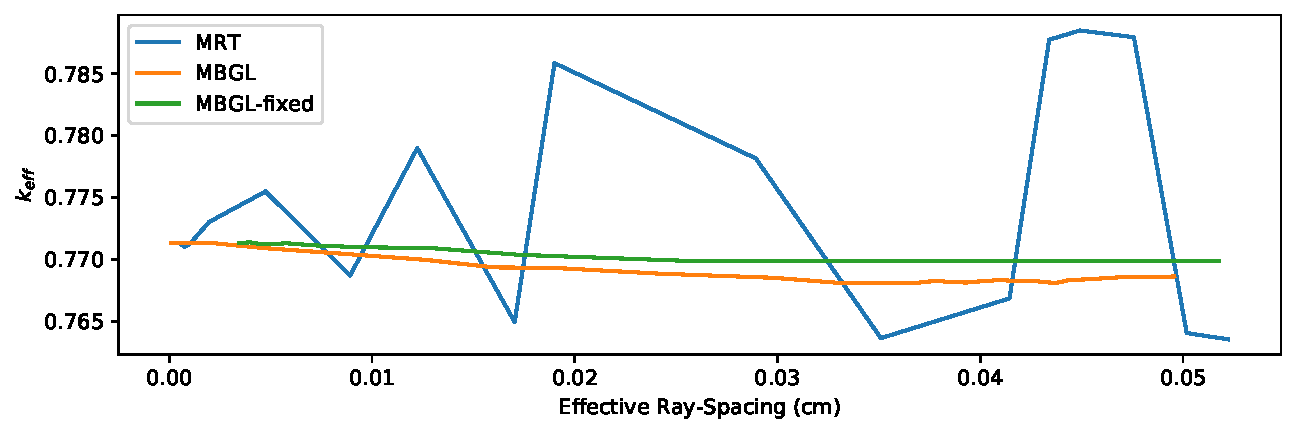
\includegraphics[width=0.95\linewidth]{\figpath/results/2D/1e/keff-vs-rayspacing}
          \caption{VERA Problem 1E: Eigenvalue results for different 2-D ray-tracing methods. \label{fig:MB:1e:keff-vs-rayspacing}}
        \end{figure}
        \begin{figure}[hp]
          \centering
          \includegraphics[width=0.95\linewidth]{\figpath/results/2D/1e/dk-vs-nSegs}
          \caption{VERA Problem 1E: Eigenvalue errors for different 2-D ray-tracing methods. \label{fig:MB:1e:dk-vs-nSegs}}
        \end{figure}
        \begin{figure}[hp]
          \centering
          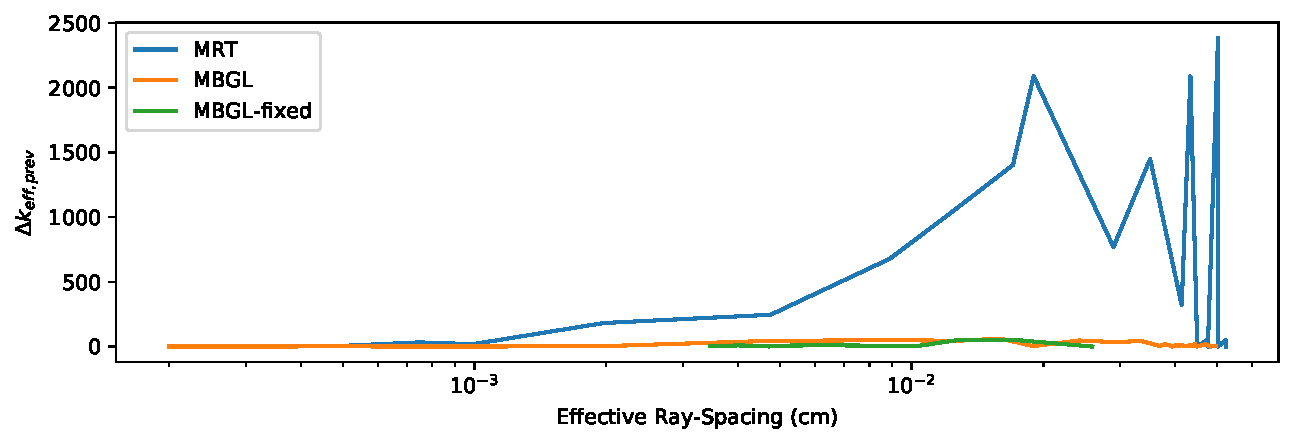
\includegraphics[width=0.95\linewidth]{\figpath/results/2D/1e/pdk-vs-rayspacing}
          \caption{VERA Problem 1E: Convergence of eigenvalue for different 2-D ray-tracing methods. \label{fig:MB:1e:pdk-vs-rayspacing}}
        \end{figure}
      }

      \subsubsection{VERA Problem 1E: 3-D}{\label{sssec:MR:1E:3-D}
        MPACT currently lacks a multigroup sweeper for 3-D self-shielding calculations, so this calculation was run without self-shielding.
        This will lead to a significantly different converged eigenvalue than for the 2-D case.
        However, even without self-shielding, this case can be used to show the benefits of the macroray ray-tracing method in 3-D \ac{MOC} calculations.
        Due to the 3-D rays, it is no longer useful to compare the results as a function of ray-spacing, as there is now the effective axial and effective radial ray-spacing.
        As it is a far better metric for the amount of work, all the 3-D results will simply use the number of track-segments for accuracy comparisons.
        Each calculation was run using od\ac{CMFD} acceleration \cite{Zhu2016}, and a directional quadrature with 64 azimuthal angles and 6 polar angles over $\fourpi$.

        \Cref{fig:MR:1e:3D:keff-vs-nSegs,fig:MR:1e:3D:pdf-vs-nSegs} show the $k$-eigenvalue as a function of the number of track segments, and the sequential differences in eigenvalue for each refinement of rays.
        These results compare the traditional \ac{MRT} method against the macroray method with a fixed number of rays in each radial and axial band (different amounts in radial and axial).
        A Gauss-Legendre quadrature was used to determine ray placement and width within each band.
        As this problem is axially homogeneous, a single ray was used in each axial band, and an axial ray-spacing of 0.75 cm was used for the \ac{MRT} method.

        These results suggest that the macroray method's ray-mesh convergence rate is higher than the traditional \ac{MRT} method's;
          the eigenvalue change between successive calculations (refining the number of rays) drops below 10 pcm with around 5.6 million segments, whereas the \ac{MRT} method was unable to converge within 10 pcm even using 14 million.
        Additionally, it is clear that the near-monotonic convergence behavior that the macroband had in 2-D holds in 3-D.

        The \ac{MRT} calculations were not continued past 14 million segments, as using finer ray-spacing resulted in significantly increased run-times, much of which was spent in the actual ray-tracing procedures.
        While the macroray does significantly simplify the ray-tracing procedure, the author believes that these long ray-tracing run-times in \ac{MRT} are likely due to unoptimized code, rather than an inherent flaw in the method.
        For 5.6 million segments, the macroray ray-tracing procedures took under 10 seconds, while for 4.8 million segments in the \ac{MRT} took 190 seconds.

        \begin{figure}[htbp]
          \centering
          \includegraphics[width=0.95\linewidth]{\figpath/results/3D/1e/keff-vs-nSegs}
          \caption{VERA Problem 1E: Eigenvalue results for different ray-tracing methods. \label{fig:MR:1e:3D:keff-vs-nSegs}}
        \end{figure}
        \begin{figure}[htbp]
          \centering
          \includegraphics[width=0.95\linewidth]{\figpath/results/3D/1e/pdk-vs-nSegs}
          \caption{VERA Problem 1E: Convergence of eigenvalue for different ray-tracing methods. \label{fig:MR:1e:3D:pdf-vs-nSegs}}
        \end{figure}
      }
    }

    \subsection{Shielded Fuel Box}{\label{ssec:MR:Shielded Fuel Box}
      The shielded fuel-box problem was created for this work to more clearly demonstrate the benefits of the macroray method for problems that pose challenges to the traditional ray-tracing methods.
      This problem consists of a 0.4$\times$0.4$\times$0.4 cm$^3$ fuel block surrounded on all sides by $0.1$ cm of a shielding material.
      This entire shielded cube is surrounded by 0.5$\times$0.5$\times$0.5 cm$^3$ cubes of moderator (26 in total).
      The calculation uses the C5G7 benchmark cross sections; the fuel is the 8.7\% \ac{MOX}, the shielding material uses the control rod cross sections.
      A 2-D cross-sectional view of the problem is shown in \cref{fig:MR:Shielded-Box Diagram}, and reflective boundary conditions are used on each face.
      This problem is meant to be similar to \ac{VERA} problem 1E, though the surrounding material was made thicker so that resolving the region did not require an extreme number of rays.

      The OpenMC Monte Carlo code \cite{OpenMC} was used to generate a reference eigenvalue to compare the results against.
      The reference solution was generated with 500 batches of 50000 particles, with 50 inactive batches.
      This yielded a reference eigenvalue with 4 pcm uncertainty.
      For MPACT, each calculation used a Chebyshev-Chebyshev directional quadrature with 24 azimuthal and 12 polar angles over $\fourpi$;
        this quadrature was chosen, rather than a Chebyshev-Gauss, as the problem has the same axial and radial descriptions.
      Similarly, the radial and axial ray-spacing used by the \ac{MRT} are the same for each calculation, and the number of rays per radial or axial band are the same.

      \begin{figure}[h]
        \centering
        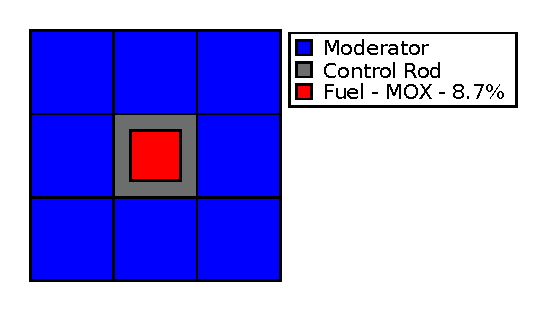
\includegraphics[width=0.75\linewidth]{\figpath/results/3D/shielded-box/ShieldedBox}
        \caption{Cross-sectional diagram of the shielded-box problem from x-y, x-z, or y-z directions. \label{fig:MR:Shielded-Box Diagram}}
      \end{figure}

      \begin{figure}[hp]
        \centering
        \includegraphics[width=0.95\linewidth]{\figpath/results/3D/shielded-box/keff-vs-nSegs}
        \caption{Shielded-Box Problem: Eigenvalue results for different 3-D ray-tracing methods. \label{fig:MR:SB:keff-vs-nSegs}}
      \end{figure}
      \begin{figure}[hp]
        \centering
        \includegraphics[width=0.95\linewidth]{\figpath/results/3D/shielded-box/dk-vs-nSegs}
        \caption{Shielded-Box Problem: Eigenvalue errors for different 3-D ray-tracing methods. \label{fig:MR:SB:dk-vs-nSegs}}
      \end{figure}
      \begin{figure}[hp]
        \centering
        \includegraphics[width=0.95\linewidth]{\figpath/results/3D/shielded-box/pdk-vs-nSegs}
        \caption{Shielded-Box Problem: Convergence of eigenvalue for different 3-D ray-tracing methods. \label{fig:MR:SB:pdk-vs-nSegs}}
      \end{figure}

      The results of the ray-tracing methods are summarized in \cref{fig:MR:SB:keff-vs-nSegs,fig:MR:SB:dk-vs-nSegs}.
      The traditional \ac{MRT} method generates very large eigenvalue errors when a coarse ray-spacing is used;
        in fact, for the first several ray-spacing values used, the eigenvalue estimate was near critical even though the reference is very sub-critical.
      This shows a major flaw in the \ac{MRT} methods, they do not consider the internal geometry and allow for such coarse spacings that the results can be entirely useless.
      In contrast, the macroray method enforces a minimum number of rays, which seems to give somewhat reasonable results.

      \Cref{fig:MR:SB:pdk-vs-nSegs} shows the change in eigenvalue for each sequential calculation (a refinement in the number of rays/segments).
      This figure also shows that for very coarse ray-spacings (resulting in near critical eigenvalues) do not have large differences in the resulting eigenvalues.
      An inexperienced user may believe that the solution is near convergence, which is certainly not the case.
      Once the ray-spacing is smaller than the thickness of the shielding, the results become reasonable.
      Although, they are still further off from the reference than the macroray method for the same number of segments.
      However, a user without knowledge of the \ac{MOC} would likely not be aware that this is a requirement of the user input.
      Although this was demonstrated with very coarse ray-spacings, a similar effect would likely be present if the shielding were thinner than the default ray-spacing of MPACT.
      This shows a clear advantage for the macroray method, in that it allows the user to more safely use the method without detailed knowledge of the method.
    }

    \subsection{C5G7}{\label{ssec:MR:C5G7}
      The C5G7 \cite{Smith2002,Smith2006} benchmarks are a set of benchmark problems commonly used to help the verification of 2-D and 3-D transport methods.
      The benchmarks provide a reference Monte Carlo solution that can be used to evaluate the accuracy of methods used to solve the problems.
      The original benchmark specified a 3-D problem, and a second benchmark reduced the axial size of this problem and added configurations with inserted control rods.
      In this work, each of the three extended 3-D benchmark problems are solved using both the traditional ray-tracing method (\ac{MRT}), and the new macroray ray-tracing method.
      \cref{figs:MR:C5G7:Layout} shows the configuration of the C5G7 core benchmark cases; the different problems differ only in their axial description.
      The radial layout of each fuel assembly is shown in \cref{fig:MR:C5G7:RadialAssemblyLayout}.

      The \ac{LSA} was used for all of the calculations in this work, and the meshing parameters used were found to be sufficient in previous studies on the \ac{LSA} \cite{Gunow2016}.
      In the axial direction, the problem was meshed into 2.38 cm slices.
      The rods (fuel, guide-tubes, and control rods), used a single radius of 0.540 cm, with 4 azimuthal divisions, and 8 azimuthal divisions in the surrounding moderator.
      The reflector pins used a radial mesh of 0.42$\times$0.42 cm$^2$.
      A Chebyshev-Gauss directional quadrature with 64 azimuthal angles and 8 polar angles over $\fourpi$ was used, as it was shown to yield good agreement in previous works with 3-D \ac{MOC} \cite{Kochunas2013}.
      A pin-wise modular ray-tracing was used, with each ray-tracing module being 1.26$\times$1.26$\times$2.38 cm$^3$.
      Convergence criteria of 1e-6 and 1e-5 were used for the eigenvalue and fission norm respectively.
      1080 spatial domains, determined by the \ac{RSB} graph-partitioning method, were used for each calculation.

      The macroray method calculations used 3 rays in each radial band and 5 rays in each axial band.
      The \ac{MRT} method calculations used 0.05 cm ray-spacing in the radial direction, and 0.15 cm in the axial direction.
      \ac{MIT} has reported that for these problems they were able to use 1.5 cm ray-spacing \cite{Gunow2016}, but in this study this was not found to be sufficient.
      This is most likely due to differences in how rays are set up within the \ac{MRT} procedures in MPACT and OpenMOC.

      Unfortunately, due to an inefficient implementation determining surface indices on parallel boundaries for 3-D \ac{MOC} in MPACT, \ac{CMFD} could not be utilized for the \ac{MRT} calculations.
      However, the time that the accelerated method would take can be estimated roughly by the ratio of iterations from the \ac{MRT} to the macrorray calculations (that used \ac{CMFD} accleration).

      \begin{figure}[htbp]
        \centering
        \begin{subfigure}[t]{0.45\textwidth}
          \centering
          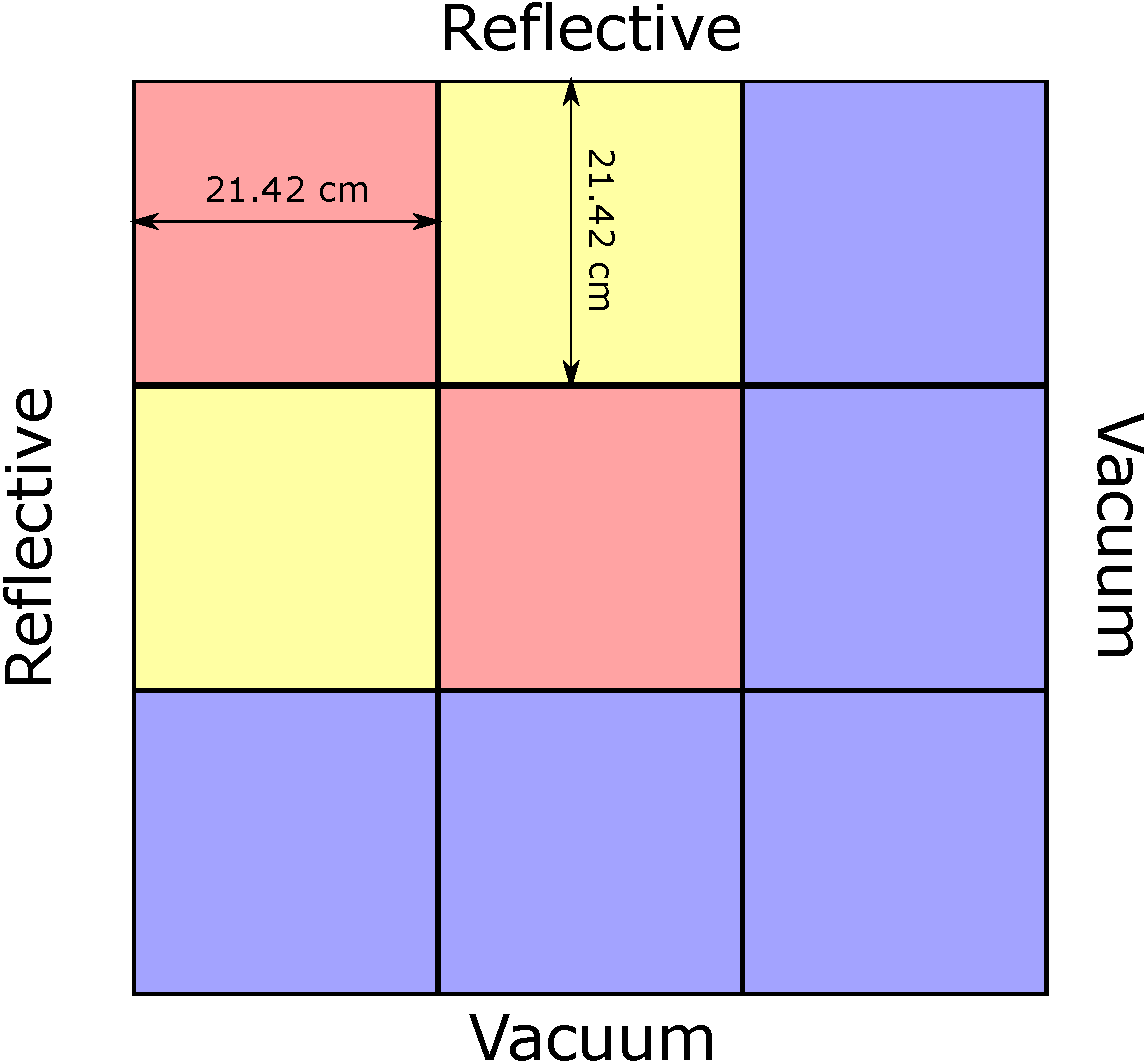
\includegraphics[width=0.9\textwidth]{\figpath/results/3D/C5G7/Diagrams/C5G7-RadialLayout}
          % \caption{\label{fig:MR:C5G7:RadialLayout}}
        \end{subfigure}%
        ~
        \begin{subfigure}[t]{0.45\textwidth}
          \centering
          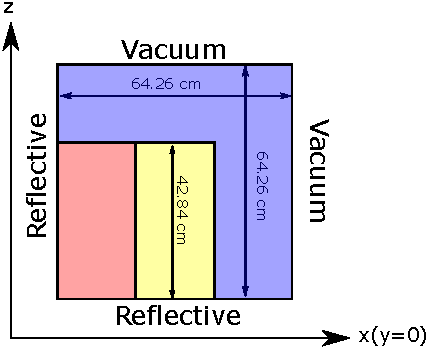
\includegraphics[width=0.9\textwidth]{\figpath/results/3D/C5G7/Diagrams/C5G7-AxialLayout}
          % \caption{fig-2\label{fig:fig-2}}
        \end{subfigure}
        \begin{subfigure}[t]{0.65\textwidth}
          \centering
          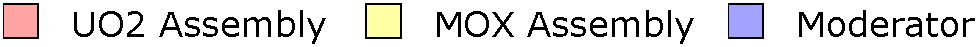
\includegraphics[width=0.9\textwidth]{\figpath/results/3D/C5G7/Diagrams/C5G7-Legend}
          % \caption{fig-2\label{fig:fig-2}}
        \end{subfigure}
        \caption{C5G7 extended benchmark core layouts. \label{figs:MR:C5G7:Layout}}
      \end{figure}

      \begin{figure}[htbp]
        \centering
        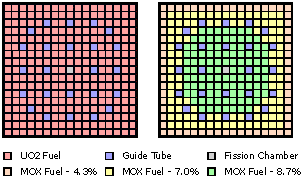
\includegraphics[width=0.85\linewidth]{\figpath/results/3D/C5G7/Diagrams/C5G7-RadialAssemblies}
        \caption{C5G7 Assembly layouts.\label{fig:MR:C5G7:RadialAssemblyLayout}}
      \end{figure}

      \subsubsection{C5G7 Benchmark: Unrodded}{\label{sssec:MR:C5G7:Unrodded}
        The unrodded case has no control rods inserted into the fuel, but control rods are present in the axial reflector region above the fuel region.
        This is shown in \cref{fig:MR:C5G7:Unrodded}.

        Eigenvalue and errors are listed in \cref{tab:MR:C5G7:Unrodded-Eigenvalues}, and pin-power results are summarized in \cref{tab:MR:C5G7:Unrodded-MRT,tab:MR:C5G7:Unrodded-MacroRay}.
        The eigenvalues for either ray-tracing method are within 100 pcm of the reference value.
        Although there is an 8 pcm difference between the two methods, this is not a significant difference.

        Overall, the macroray method results in better pin-power comparisons in each metric except for slightly higher error in the maximum pin-power.
        Additionally, the number of pins within the uncertainty levels of the reference is much higher for the macroray method, indicating better overall predictions in pin-power.
        However, the macroray method seems to have a bias in the top 1/3 of the fuel, where the power level is lower.
        The pin-power comparisons within this axial level are significantly worse than in the lower 2/3.

        \begin{table}[htbp]
          \centering
          \caption{C5G7 Benchmark: Unrodded eigenvalue comparisons. \label{tab:MR:C5G7:Unrodded-Eigenvalues}}
          \begin{tabular}{rrr}\toprule
            Case & Eigenvalue & Error (pcm)\\\midrule
            Reference & 1.143080 & $\pm$ 7\\
            MRT       & 1.142453 & -63\\
            MacroRay  & 1.142366 & -71\\\bottomrule
          \end{tabular}
        \end{table}

        \begin{figure}[htbp]
          \centering
          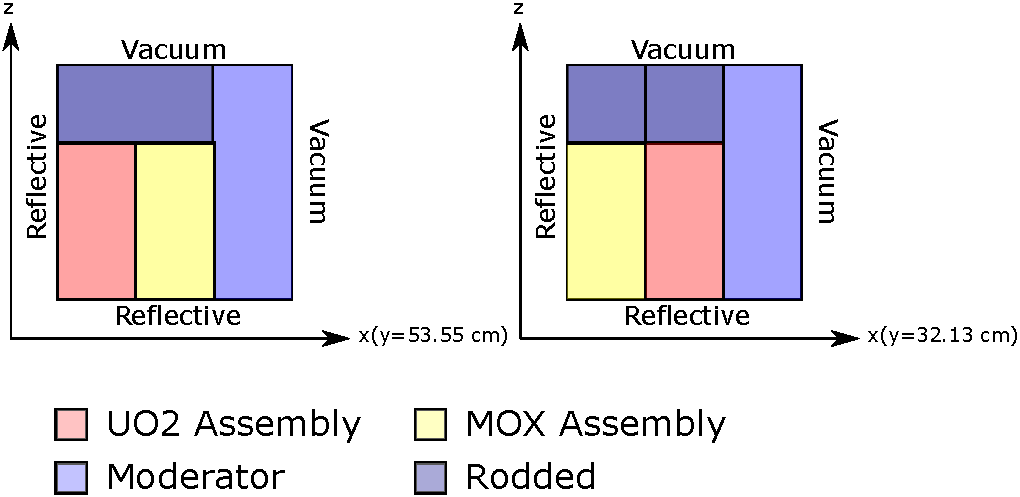
\includegraphics[width=0.85\linewidth]{\figpath/results/3D/C5G7/Diagrams/C5G7-Unrodded}
          \caption{C5G7 Benchmark: Unrodded core configuration. \label{fig:MR:C5G7:Unrodded}}
        \end{figure}

        \begin{table}[htbp]
          \centering
          \caption{C5G7 Benchmark: Unrodded pin-power comparisons for the MRT method. \label{tab:MR:C5G7:Unrodded-MRT}}
          \scriptsize
          \begin{tabular}{rrrrrrrrr}\toprule
                                  & \multicolumn{2}{c}{Z Slice \# 1} & \multicolumn{2}{c}{Z Slice \# 2} & \multicolumn{2}{c}{Z Slice \# 3} & \multicolumn{2}{c}{Overall}\\
                                  & Reference & MRT & Reference & MRT & Reference & MRT & Reference & MRT\\\midrule
            Maximum Pin Power     & 1.108 & 1.107 & 0.882 & 0.881 & 0.491 & 0.488 & 2.481 & 2.476\\
            Percent Error         & 0.090 & -0.093 & 0.100 & -0.184 & 0.130 & -0.545 & 0.060 & -0.215\\\midrule
            Maximum Error         & 0.290 & 2.483 & 0.320 & 2.538 & 0.430 & 2.618 & 0.192 & 2.454\\
            AVG Error             & 0.164 & 0.354 & 0.183 & 0.358 & 0.245 & 0.363 & 0.109 & 0.329\\
            RMS Error             & 0.171 & 0.522 & 0.190 & 0.518 & 0.255 & 0.505 & 0.114 & 0.486\\
            MRE Error             & 0.062 & 0.114 & 0.055 & 0.094 & 0.042 & 0.058 & 0.093 & 0.241\\\midrule
            \# Pins within 68\%   & 371 & 177 & 371 & 197 & 371 & 234 & 371 & 142\\
            \# Pins within 95\%   & 518 & 323 & 518 & 335 & 518 & 392 & 518 & 248\\
            \# Pins within 99\%   & 540 & 388 & 540 & 414 & 540 & 457 & 540 & 310\\
            \# Pins within 99.9\% & 544 & 438 & 544 & 456 & 544 & 499 & 544 & 368\\\midrule
            UO2-1 Power           & 219.04 & 218.63 & 174.24 & 173.91 & 97.93 & 97.73 & 491.21 & 490.27\\
            MOX Power             & 94.53 & 94.61 & 75.25 & 75.27 & 42.92 & 42.97 & 212.70 & 212.85\\
            UO2-2 Power           & 62.12 & 62.43 & 49.45 & 49.68 & 27.82 & 27.91 & 139.39 & 140.02\\
            UO2-1 Power \% Error  & 0.082 & -0.185 & 0.073 & -0.188 & 0.055 & -0.212 & 0.123 & -0.192\\
            MOX Power \% Error    & 0.061 & 0.082 & 0.054 & 0.032 & 0.041 & 0.116 & 0.092 & 0.071\\
            UO2-2 Power \% Error  & 0.043 & 0.508 & 0.038 & 0.466 & 0.029 & 0.334 & 0.065 & 0.458\\\bottomrule
          \end{tabular}
        \end{table}

        \begin{table}[htbp]
          \centering
          \caption{C5G7 Benchmark: Unrodded pin-power comparisons for the macroray method. \label{tab:MR:C5G7:Unrodded-MacroRay}}
          \scriptsize
          \begin{tabular}{rrrrrrrrr}\toprule
                                  & \multicolumn{2}{c}{Z Slice \# 1} & \multicolumn{2}{c}{Z Slice \# 2} & \multicolumn{2}{c}{Z Slice \# 3} & \multicolumn{2}{c}{Overall}\\
                                  & Reference & MacroRay & Reference & MacroRay & Reference & MacroRay & Reference & MacroRay\\\midrule
            Maximum Pin Power     & 1.108 & 1.105 & 0.882 & 0.880 & 0.491 & 0.491 & 2.481 & 2.475\\
            Percent Error         & 0.090 & -0.331 & 0.100 & -0.309 & 0.130 & 0.108 & 0.060 & -0.236\\\midrule
            Maximum Error         & 0.280 & 0.862 & 0.250 & 1.131 & 0.330 & 2.014 & 0.192 & 0.910\\
            AVG Error             & 0.164 & 0.257 & 0.183 & 0.235 & 0.245 & 0.830 & 0.109 & 0.190\\
            RMS Error             & 0.171 & 0.300 & 0.190 & 0.294 & 0.255 & 0.902 & 0.114 & 0.248\\
            MRE Error             & 0.062 & 0.130 & 0.055 & 0.083 & 0.042 & 0.149 & 0.093 & 0.161\\\midrule
            \# Pins within 68\%   & 371 & 188 & 371 & 229 & 371 & 9 & 371 & 180\\
            \# Pins within 95\%   & 518 & 328 & 518 & 396 & 518 & 74 & 518 & 342\\
            \# Pins within 99\%   & 540 & 399 & 540 & 462 & 540 & 132 & 540 & 411\\
            \# Pins within 99.9\% & 544 & 441 & 544 & 508 & 544 & 232 & 544 & 480\\\midrule
            UO2-1 Power           & 219.04 & 218.21 & 174.24 & 173.79 & 97.93 & 98.48 & 491.21 & 490.47\\
            MOX Power             & 94.53 & 94.40 & 75.25 & 75.23 & 42.92 & 43.33 & 212.70 & 212.97\\
            UO2-2 Power           & 62.12 & 62.09 & 49.45 & 49.48 & 27.82 & 28.03 & 139.39 & 139.59\\
            UO2-1 Power \% Error  & 0.082 & -0.380 & 0.073 & -0.259 & 0.055 & 0.554 & 0.123 & -0.151\\
            MOX Power \% Error    & 0.061 & -0.134 & 0.054 & -0.021 & 0.041 & 0.957 & 0.092 & 0.126\\
            UO2-2 Power \% Error  & 0.043 & -0.047 & 0.038 & 0.053 & 0.029 & 0.744 & 0.065 & 0.147\\\bottomrule
          \end{tabular}
        \end{table}

        \Cref{tab:MR:C5G7:Unrodded-Performance} lists the total run-time of each calculation.
        The \ac{MRT} calculation took 911 iterations to converge (unaccelerated), while the macroray method took 30 to converge.
        This gives an estimate for the accelerated \ac{MRT} method at 240 core-hours.
        Unfortunately, this is quite significantly better in terms of run-time than the macroray method.
        A further discussion of this will be presented in \cref{sec:Discussion one the Performance of MacroRay}.

        \begin{table}[htbp]
          \centering
          \caption{C5G7 Benchmark: Unrodded Performance. \label{tab:MR:C5G7:Unrodded-Performance}}
          \begin{tabular}{rrr}\toprule
            Case                        & Acclerated? & Time (core-hours)\\\midrule
            LSMoC - MRT                 & F & 7293\\
            LSMoC - MacroRay            & T & 618\\\bottomrule
          \end{tabular}
        \end{table}


        By refining the axial mesh height the accuracy of the macroray calculations can be increased.
        The previous mesh used an axial source region height of 2.38 cm; by using a height of 1.785 cm, the eigenvalue error is reduced to -54 pcm.
        By further reducing to an axial source height of 1.428 cm the eigenvalue error becomes -49 pcm.
        While a similar study was not performed on the rodded B case, the same trend is expected.
      }

      \subsubsection{C5G7 Benchmark: Rodded A}{\label{sssec:MR:C5G7:Rodded A}
        The C5G7 rodded A case has control rods partially inserted 14.28 cm, one third of the fuel height, into the central \ac{UO2} assembly.
        The remaining \ac{UO2} assembly and \ac{MOX} assemblies have no inserted control rods.
        The core layout is depicted in \cref{fig:MR:C5G7:Rodded A}.

        Eigenvalue and errors are listed in \cref{tab:MR:C5G7:Rodded A-Eigenvalues}, and pin-power results are summarized in \cref{tab:MR:C5G7:Rodded A-MRT,tab:MR:C5G7:Rodded A-MacroRay}.
        Similarly to the unrodded case, the eigenvalues for each ray-tracing method are within 100 pcm; however, the error is 34 pcm higher for the macroray method.
        Again, in overall pin-power comparisons, the macroray method outperforms the MRT method in all except the error in the maximum pin-power.
        Additionally, the number of pins predicted within the uncertainty levels of the reference are significantly higher for the macroray method.
        But, just like in the unrodded case, the macroray method performs significantly worse in the low-power upper third of the fuel.

        \begin{figure}[htbp]
          \centering
          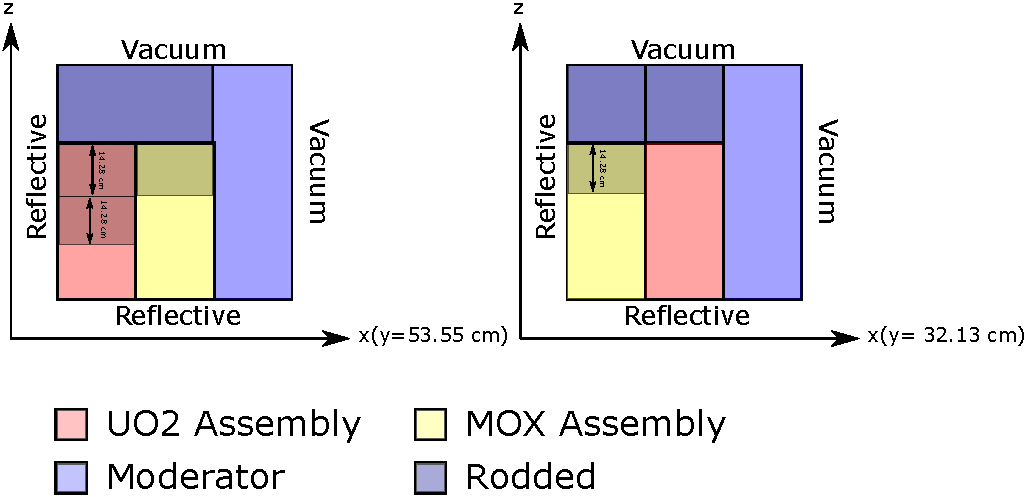
\includegraphics[width=0.85\linewidth]{\figpath/results/3D/C5G7/Diagrams/C5G7-RoddedB}
          \caption{C5G7 Benchmark: Rodded A core configuration. \label{fig:MR:C5G7:Rodded A}}
        \end{figure}

        \begin{table}[htbp]
          \centering
          \caption{C5G7 Benchmark: Rodded A eigenvalue comparisons. \label{tab:MR:C5G7:Rodded A-Eigenvalues}}
          \begin{tabular}{rrr}\toprule
            Case & Eigenvalue & Error (pcm)\\\midrule
            Reference & 1.128060 & $\pm$ 7\\
            MRT       & 1.127585 & -47\\
            MacroRay  & 1.127248 & -81\\\bottomrule
          \end{tabular}
        \end{table}

        \begin{table}[htbp]
          \centering
          \caption{C5G7 Benchmark: Rodded A pin-power comparisons for the MRT method. \label{tab:MR:C5G7:Rodded A-MRT}}
          \scriptsize
          \begin{tabular}{rrrrrrrrr}\toprule
                                  & \multicolumn{2}{c}{Z Slice \# 1} & \multicolumn{2}{c}{Z Slice \# 2} & \multicolumn{2}{c}{Z Slice \# 3} & \multicolumn{2}{c}{Overall}\\
                                  & Reference & MRT & Reference & MRT & Reference & MRT & Reference & MRT\\\midrule
            Maximum Pin Power     & 1.197 & 1.198 & 0.832 & 0.830 & 0.304 & 0.300 & 2.253 & 2.249\\
            Percent Error         & 0.080 & 0.085 & 0.100 & -0.151 & 0.200 & -1.237 & 0.059 & -0.211\\\midrule
            Maximum Error         & 0.270 & 1.948 & 0.310 & 2.168 & 0.180 & 2.014 & 0.183 & 1.934\\
            AVG Error             & 0.157 & 0.429 & 0.180 & 0.334 & 0.260 & 0.837 & 0.108 & 0.294\\
            RMS Error             & 0.163 & 0.566 & 0.186 & 0.471 & 0.266 & 0.962 & 0.111 & 0.430\\
            MRE Error             & 0.066 & 0.156 & 0.056 & 0.093 & 0.037 & 0.146 & 0.094 & 0.220\\\midrule
            \# Pins within 68\%   & 371 & 106 & 371 & 197 & 371 & 93 & 371 & 151\\
            \# Pins within 95\%   & 518 & 237 & 518 & 350 & 518 & 175 & 518 & 270\\
            \# Pins within 99\%   & 540 & 312 & 540 & 415 & 540 & 223 & 540 & 338\\
            \# Pins within 99.9\% & 544 & 386 & 544 & 471 & 544 & 281 & 544 & 391\\\midrule
            UO2-1 Power           & 237.41 & 237.80 & 167.51 & 167.23 & 56.26 & 55.47 & 461.18 & 460.49\\
            MOX Power             & 104.48 & 104.85 & 78.01 & 77.99 & 39.23 & 38.95 & 221.71 & 221.78\\
            UO2-2 Power           & 69.80 & 70.22 & 53.39 & 53.58 & 28.21 & 28.14 & 151.39 & 151.94\\
            UO2-1 Power \% Error  & 0.087 & 0.164 & 0.071 & -0.170 & 0.040 & -1.404 & 0.119 & -0.149\\
            MOX Power \% Error    & 0.065 & 0.351 & 0.056 & -0.022 & 0.040 & -0.716 & 0.094 & 0.031\\
            UO2-2 Power \% Error  & 0.047 & 0.608 & 0.040 & 0.356 & 0.029 & -0.232 & 0.068 & 0.363\\\bottomrule
          \end{tabular}
        \end{table}

        \begin{table}[htbp]
          \centering
          \caption{C5G7 Benchmark: Rodded A pin-power comparisons for the macrorray method. \label{tab:MR:C5G7:Rodded A-MacroRay}}
          \scriptsize
          \begin{tabular}{rrrrrrrrr}\toprule
                                  & \multicolumn{2}{c}{Z Slice \# 1} & \multicolumn{2}{c}{Z Slice \# 2} & \multicolumn{2}{c}{Z Slice \# 3} & \multicolumn{2}{c}{Overall}\\
                                  & Reference & MacroRay & Reference & MacroRay & Reference & MacroRay & Reference & MacroRay\\\midrule
            Maximum Pin Power     & 1.197 & 1.190 & 0.832 & 0.828 & 0.304 & 0.307 & 2.253 & 2.245\\
            Percent Error         & 0.080 & -0.542 & 0.100 & -0.387 & 0.200 & 1.088 & 0.059 & -0.387\\\midrule
            Maximum Error         & 0.210 & 0.976 & 0.240 & 1.120 & 0.350 & 1.881 & 0.143 & 0.985\\
            AVG Error             & 0.157 & 0.240 & 0.180 & 0.256 & 0.260 & 0.937 & 0.108 & 0.222\\
            RMS Error             & 0.163 & 0.288 & 0.186 & 0.320 & 0.266 & 0.986 & 0.111 & 0.275\\
            MRE Error             & 0.066 & 0.136 & 0.056 & 0.091 & 0.037 & 0.140 & 0.094 & 0.198\\\midrule
            \# Pins within 68\%   & 371 & 212 & 371 & 229 & 371 & 8 & 371 & 145\\
            \# Pins within 95\%   & 518 & 341 & 518 & 369 & 518 & 38 & 518 & 272\\
            \# Pins within 99\%   & 540 & 390 & 540 & 429 & 540 & 100 & 540 & 360\\
            \# Pins within 99.9\% & 544 & 433 & 544 & 490 & 544 & 194 & 544 & 439\\\midrule
            UO2-1 Power           & 237.41 & 236.50 & 167.51 & 167.00 & 56.26 & 56.74 & 461.18 & 460.24\\
            MOX Power             & 104.48 & 104.40 & 78.01 & 78.04 & 39.23 & 39.61 & 221.71 & 222.04\\
            UO2-2 Power           & 69.80 & 69.76 & 53.39 & 53.46 & 28.21 & 28.45 & 151.39 & 151.67\\
            UO2-1 Power \% Error  & 0.087 & -0.382 & 0.071 & -0.305 & 0.040 & 0.855 & 0.119 & -0.203\\
            MOX Power \% Error    & 0.065 & -0.077 & 0.056 & 0.040 & 0.040 & 0.972 & 0.094 & 0.150\\
            UO2-2 Power \% Error  & 0.047 & -0.050 & 0.040 & 0.128 & 0.029 & 0.849 & 0.068 & 0.180\\\bottomrule
          \end{tabular}
        \end{table}

        \Cref{tab:MR:C5G7:Rodded A-Performance} lists the total run-time of each calculation.
        The \ac{MRT} calculation took 936 iterations to converge (unaccelerated), while the macroray method took 31 to converge.
        This gives an estimate for the accelerated \ac{MRT} method at 246 core-hours.
        Again, this is much better than how the macroray method performed.

        \begin{table}[htbp]
          \centering
          \caption{C5G7 Benchmark: Rodded A Performance. \label{tab:MR:C5G7:Rodded A-Performance}}
          \begin{tabular}{rrr}\toprule
            Case                        & Acclerated? & Time (core-hours)\\\midrule
            LSMoC - MRT                 & F &  7433\\
            LSMoC - MacroRay            & T &   587\\\bottomrule
          \end{tabular}
        \end{table}
      }

      \subsubsection{C5G7 Benchmark: Rodded B}{\label{sssec:MR:C5G7:Rodded B}
        The C5G7 rodded B case has control rods partially inserted into three of the four fuel assemblies.
        Each of the \ac{MOX} assemblies has control rods inserted 14.28 cm.
        The center \ac{UO2} assembly has control rods inserted 28.56 cm, two thirds of the fuel height; the outer \ac{UO2} assembly has no inserted control rods.
        This layout is depicted in \cref{fig:MR:C5G7:Rodded B}.

        Eigenvalue and errors are listed in \cref{tab:MR:C5G7:Rodded B-Eigenvalues}, and pin-power results are summarized in \cref{tab:MR:C5G7:Rodded B-MRT,tab:MR:C5G7:Rodded B-MacroRay}.
        In this case, the macroray method yields eigenvalue error just over 100 pcm, while the \ac{MRT} method is well under 100.
        The difference in eigenvalue error is likely primarily due to the fact that the \ac{MRT} benefits from cancellation of errors, while the macrorray generally does not.

        Interestingly, the overall pin-power comparisons are much closer in this case compared to the unrodded and rodded A configurations.
        The average, RMS and mean relative errors are all similar compared to the \ac{MRT} method; the error in the maximum power is higher for the macroray method, just as in the previous cases.
        The macroray method also does not outperform the \ac{MRT} method in the number of pins within each uncertainty level of the reference.
        Finally, the macroray method again shows the most significant errors in the upper 1/3 of the fuel, as in previous cases.
        As mentioned in \cref{sssec:MR:C5G7:Unrodded}, if the axial mesh was refined, lower errors would be expected.

        \begin{figure}[htbp]
          \centering
          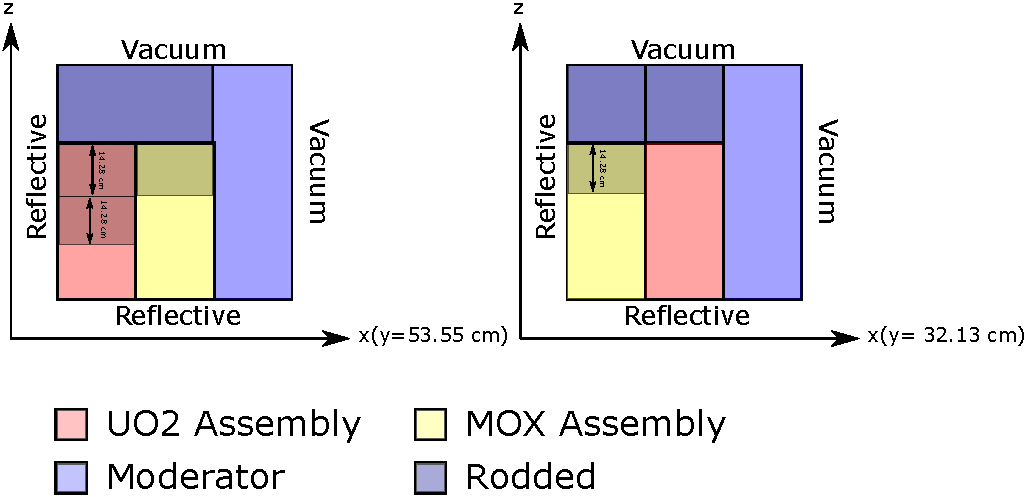
\includegraphics[width=0.85\linewidth]{\figpath/results/3D/C5G7/Diagrams/C5G7-RoddedB}
          \caption{C5G7 Benchmark: Rodded B core configuration. \label{fig:MR:C5G7:Rodded B}}
        \end{figure}

        \begin{table}[htbp]
          \centering
          \caption{C5G7 Benchmark: Rodded B eigenvalue comparisons. \label{tab:MR:C5G7:Rodded B-Eigenvalues}}
          \begin{tabular}{rrr}\toprule
            Case & Eigenvalue & Error (pcm)\\\midrule
            Reference & 1.077770 & $\pm$ 7\\
            MRT       & 1.077268  & -50\\
            MacroRay  & 1.076628 & -114\\\bottomrule
          \end{tabular}
        \end{table}

        \begin{table}[htbp]
          \centering
          \caption{C5G7 Benchmark: Unrodded pin-power comparisons for the MRT method. \label{tab:MR:C5G7:Rodded B-MRT}}
          \scriptsize
          \begin{tabular}{rrrrrrrrr}\toprule
                                  & \multicolumn{2}{c}{Z Slice \# 1} & \multicolumn{2}{c}{Z Slice \# 2} & \multicolumn{2}{c}{Z Slice \# 3} & \multicolumn{2}{c}{Overall}\\
                                  & Reference & MRT & Reference & MRT & Reference & MRT & Reference & MRT\\\midrule
            Maximum Pin Power     & 1.200 & 1.208 & 0.554 & 0.549 & 0.217 & 0.211 & 1.835 & 1.834\\
            Percent Error         & 0.090 & 0.691 & 0.150 & -0.909 & 0.240 & -2.738 & 0.083 & -0.065\\\midrule
            Maximum Error         & 0.240 & 2.449 & 0.270 & 1.641 & 0.240 & 2.738 & 0.163 & 1.850\\
            AVG Error             & 0.146 & 0.639 & 0.181 & 0.546 & 0.285 & 1.593 & 0.105 & 0.251\\
            RMS Error             & 0.150 & 0.730 & 0.184 & 0.619 & 0.290 & 1.712 & 0.108 & 0.366\\
            MRE Error             & 0.073 & 0.348 & 0.055 & 0.183 & 0.034 & 0.208 & 0.098 & 0.203\\\midrule
            \# Pins within 68\%   & 371 & 28 & 371 & 78 & 371 & 25 & 371 & 167\\
            \# Pins within 95\%   & 518 & 83 & 518 & 161 & 518 & 61 & 518 & 308\\
            \# Pins within 99\%   & 540 & 124 & 540 & 225 & 540 & 80 & 540 & 375\\
            \# Pins within 99.9\% & 544 & 183 & 544 & 290 & 544 & 110 & 544 & 427\\\midrule
            UO2-1 Power           & 247.75 & 249.43 & 106.56 & 105.72 & 41.12 & 40.23 & 395.43 & 395.38\\
            MOX Power             & 125.78 & 126.48 & 81.41 & 81.09 & 29.42 & 28.94 & 236.62 & 236.51\\
            UO2-2 Power           & 91.64 & 92.22 & 65.02 & 65.02 & 30.68 & 30.36 & 187.34 & 187.60\\
            UO2-1 Power \% Error  & 0.091 & 0.681 & 0.056 & -0.791 & 0.035 & -2.180 & 0.112 & -0.013\\
            MOX Power \% Error    & 0.073 & 0.556 & 0.058 & -0.394 & 0.034 & -1.635 & 0.100 & -0.043\\
            UO2-2 Power \% Error  & 0.055 & 0.636 & 0.046 & -0.010 & 0.032 & -1.046 & 0.078 & 0.137\\\bottomrule
          \end{tabular}
        \end{table}

        \begin{table}[htbp]
          \centering
          \caption{C5G7 Benchmark: Rodded B pin-power comparisons for the macroray method. \label{tab:MR:C5G7:Rodded B-MacroRay}}
          \scriptsize
          \begin{tabular}{rrrrrrrrr}\toprule
                                  & \multicolumn{2}{c}{Z Slice \# 1} & \multicolumn{2}{c}{Z Slice \# 2} & \multicolumn{2}{c}{Z Slice \# 3} & \multicolumn{2}{c}{Overall}\\
                                  & Reference & MacroRay & Reference & MacroRay & Reference & MacroRay & Reference & MacroRay\\\midrule
            Maximum Pin Power     & 1.200 & 1.190 & 0.554 & 0.553 & 0.217 & 0.219 & 1.835 & 1.831\\
            Percent Error         & 0.090 & -0.801 & 0.150 & -0.128 & 0.240 & 0.832 & 0.083 & -0.215\\\midrule
            Maximum Error         & 0.100 & 0.925 & 0.240 & 1.207 & 0.370 & 2.771 & 0.157 & 1.100\\
            AVG Error             & 0.146 & 0.329 & 0.181 & 0.216 & 0.285 & 1.322 & 0.105 & 0.222\\
            RMS Error             & 0.150 & 0.391 & 0.184 & 0.291 & 0.290 & 1.367 & 0.108 & 0.290\\
            MRE Error             & 0.073 & 0.225 & 0.055 & 0.060 & 0.034 & 0.160 & 0.098 & 0.203\\\midrule
            \# Pins within 68\%   & 371 & 133 & 371 & 286 & 371 & 1 & 371 & 172\\
            \# Pins within 95\%   & 518 & 268 & 518 & 444 & 518 & 3 & 518 & 288\\
            \# Pins within 99\%   & 540 & 332 & 540 & 501 & 540 & 14 & 540 & 342\\
            \# Pins within 99.9\% & 544 & 385 & 544 & 530 & 544 & 65 & 544 & 405\\\midrule
            UO2-1 Power           & 247.75 & 246.26 & 106.56 & 106.63 & 41.12 & 41.63 & 395.43 & 394.51\\
            MOX Power             & 125.78 & 125.56 & 81.41 & 81.48 & 29.42 & 29.84 & 236.62 & 236.89\\
            UO2-2 Power           & 91.64 & 91.55 & 65.02 & 65.15 & 30.68 & 31.02 & 187.34 & 187.71\\
            UO2-1 Power \% Error  & 0.091 & -0.600 & 0.056 & 0.063 & 0.035 & 1.227 & 0.112 & -0.231\\
            MOX Power \% Error    & 0.073 & -0.179 & 0.058 & 0.095 & 0.034 & 1.423 & 0.100 & 0.115\\
            UO2-2 Power \% Error  & 0.055 & -0.104 & 0.046 & 0.192 & 0.032 & 1.120 & 0.078 & 0.199\\\bottomrule
          \end{tabular}
        \end{table}

        \Cref{tab:MR:C5G7:Rodded B-Performance} lists the total run-time of each calculation.
        The \ac{MRT} calculation took 933 iterations to converge (unaccelerated), while the macroray method took 30 to converge.
        This gives an estimate for the accelerated \ac{MRT} method at 241 core-hours.
        Just as the previous two cases, this is significantly lower than the time the macroray method took.

        \begin{table}[htbp]
          \centering
          \caption{C5G7 Benchmark: Rodded B Performance. \label{tab:MR:C5G7:Rodded B-Performance}}
          \begin{tabular}{rrr}\toprule
            Case                        & Acclerated? & Time (core-hours)\\\midrule
            LSMoC - MRT                 & F & 7493\\
            LSMoC - MacroRay            & T & 579\\\bottomrule
          \end{tabular}
        \end{table}
      }
    }
  }

  \section{Discussion on the Performance of MacroRay}{\label{sec:Discussion one the Performance of MacroRay}
    While the macroray method was able to reduce the number of segments in some cases, macroray calculations generally took longer for the same number of segments compared to the \ac{MRT} method.
    To determine where the performance was lacking, a miniaturized C5G7 unrodded case was profiled, without using \ac{CMFD} acceleration, and with 18 spatial domains, using both the \ac{MRT} and macroray methods.
    For each calculation, nearly all the time was spent in the transport routines ($>$95\%).
    The transmission calculations and moment accumulation are typically the largest run-time contributors in \ac{MRT} calculations, and the profiler revealed that 61.8\% of the time was spent in these loops.
    An additional 33\% was spent on waiting for messages from other domains.

    The \acf{MPI} \cite{MPI} is a standard for communication in distributed computations that communicates data by passing messages between computational nodes; it was used by this work for communication between spatial subdomains.
    Messages require information about the size of the message, data type, data buffer, and a tag that uniquely identifies the message.
    The data passing between spatial domains was accomplished using asynchronous messages, where multiple messages may be queued for sending/receiving while the program continues running until a wait or waitall call.

    In the macroray calculation, only 22\% of the total time was spent in the transmission and accumulation loops and 15.1 \% was spent on the conversion between ray fluxes and surface fluxes.
    The largest contributor to run-time was waiting for MPI messages, at 57.4\%.
    In the current implementation, a MPI waitall command is used after sweeping each direction.
    The fractional run-time can be reduced to 26\% if the waitall is moved to after sweeping all directions.
    This is the same approach used by the \ac{MRT} sweepers in MPACT.
    However, the method of generating unique message tags must be improved for the macrorray sweepers, because the current method results in a tag overflow on larger cases such as the C5G7 benchmarks.

    While the conversion between ray and surface fluxes will never be zero, it is unlikely that the naive implementation of these routines in this work are nearly optimal.
    A better implementation of these routines may significantly cut down on run-time costs.
  }


  \section{Conclusions}{\label{sec:MR:Conclusions}
    The macroray method was motivated by previous studies on the macroband method that claimed significantly reduced number of rays with maintained accuracy.
    It was expected that the method, if extended to 3-D, would allow for significantly fewer track-segments, and thus lead to less computational work.
    For some problems, this is certainly the case; for \ac{VERA} progression problem 1E, a single \ac{IFBA} rod, this method was able to significantly reduce the number of segments to reach a converged result.
    Additionally, for the shielded-box problem, this method is able to act as more of a ``black box'' solver, allowing for users without deep knowledge of the method to use it.

    The method was then tested on the extended 3-D C5G7 benchmarks, and proved it was able to handle larger calculations.
    Compared to the \ac{MRT} method on the same mesh, the macroray method typically better-predicted the pin-powers, even when eigenvalue errors were larger.
    Additionally, the macroray method consistently showed the highest errors in the upper 1/3 of the fuel in the C5G7 benchmark cases, where the pin-powers are lower.

    In the C5G7 benchmark cases, which do not have small absorber regions, the method was unable to significantly reduce the number of segments for similar accuracy.
    It is expected that the macroray method may show more beneficial results in cases where there are small strong absorber regions present.
    Additionally, the macroray method may show significant benefits for more arbitrary geometries, such as the shielded-box.

    This work is the first implementation of the macroray method for 3-D \ac{MOC} calculations.
    Due to the significantly different ray-tracing data structure, and sweeping order, separate routines needed to be written for this work.
    It is not surprising that the initial performance of these routines is worse than that of the \ac{MRT}-based routines, for similar numbers of segments, given that the \ac{MRT} sweeping routines have been optimized over the past several years of the \ac{CASL} project.
    The original performance of the 3-D \ac{MOC} using \ac{MRT} in MPACT was significantly worse \cite{Kochunas2013}.
    While some of the improvements made to these methods were utilized in this work, it is very likely that optimization work on this method would significantly reduce run-times.
  }
  % References
  \printbibliography
}